\chapter{Applicability}
% informal description of target / story -> show that it makes sense
% Use Cases, not concrete
We have introduced a conceptual model for reactive information systems and its services.
In this chapter we will show how this model applies to certain use cases.

\section{Augment existing Web Applications}
\index{CMS}
Web applications, such as webmails, social networks or content management systems (\textrm{CMS}) are widely spread and used by a large number of internet users.
But often users ord developer miss some features or interoperability with other web applications, which would result in augmented functionality and also in less work.
Features of that kind could also include data and functionality from other sites on the web.
This would require web applications to mashup together and to grab data or invoke functionality on each other.
Many kinds of augmentations will not be implemented by the web applications themselves because they are very specific to a small number of their users.
With a reactive information system, users and developers could realize such features on their own.

\subsection{Enrich \textrm{CMS} Posts with Additional Information}
Every new post to a content management system can be modeled as an event.
In the case that a user would like to enrich such a system with founded knowledge from a remote resource, reactivity in the Web can be used to enrich it.
Augmenting an existing \textrm{CMS} can be realized by a rule that evaluates new posts and checks whether knowledge tags are included in the post.
Whenever there are tags included within the post, the reactive system will enrich the post with additional knowledge to these tags from a remote service of the user's choice.
\begin{figure}[!ht]
  \centering
  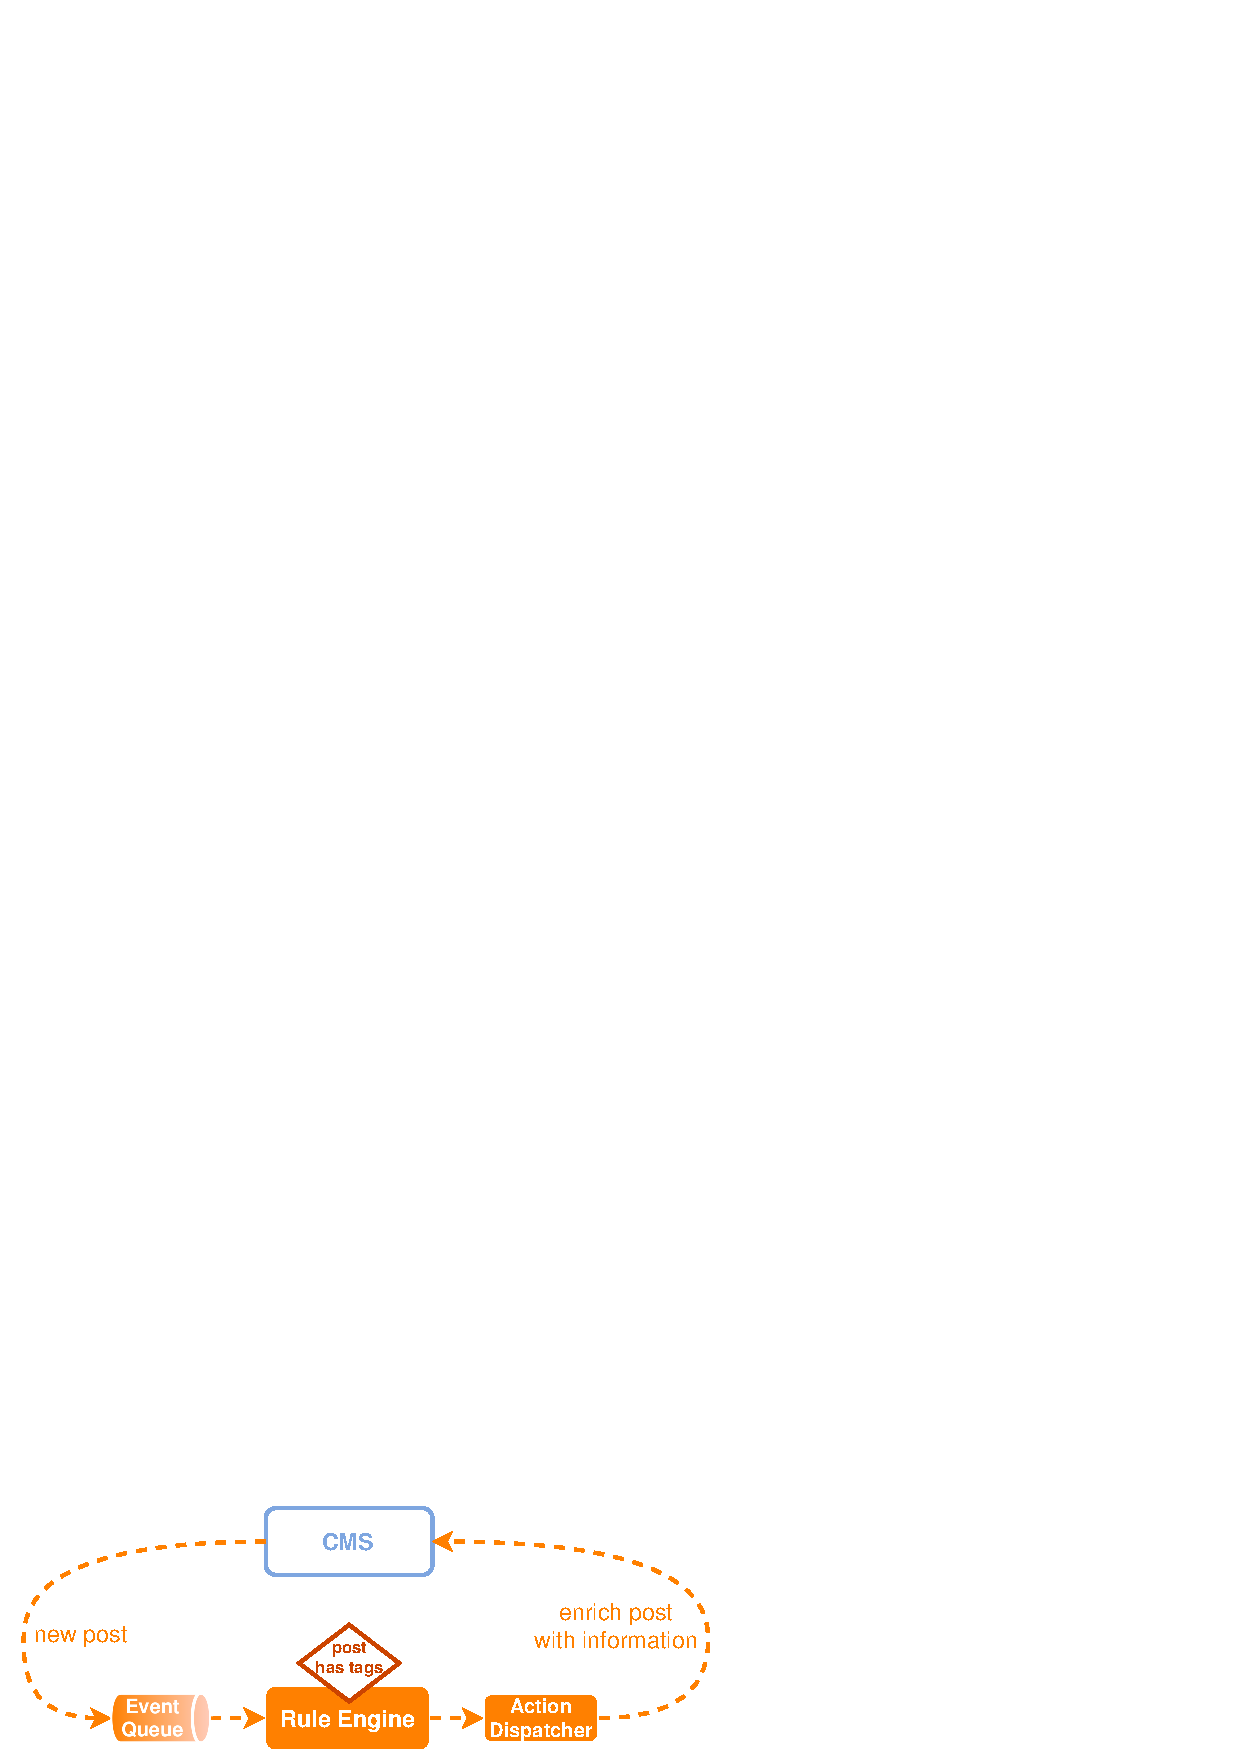
\includegraphics{figures/ProBinderAnnotations}
  \caption{Enrich CMS Post with Remote Knowledge Data}
  \label{fig:ProBinderAnnotations}
\end{figure}

\subsection{Workflow Automation}
Within such web applications, users often have very specific workflows.
And because workflows always start with an event, they are predestinated to be automated by a reactive information system.
As an example for workflow automation, course and student exercise submission administration can be taken care of by a reactive information system.
Whenever a new semester starts, the reactive system will detect this through one of its rules and command an action dispatcher to set up infrastructures for courses.
This can also include grabbing course data from an official web page and including it into the infrastrucutre, thus eliminating the need for manual data copy tasks.
\begin{figure}[!ht]
  \centering
  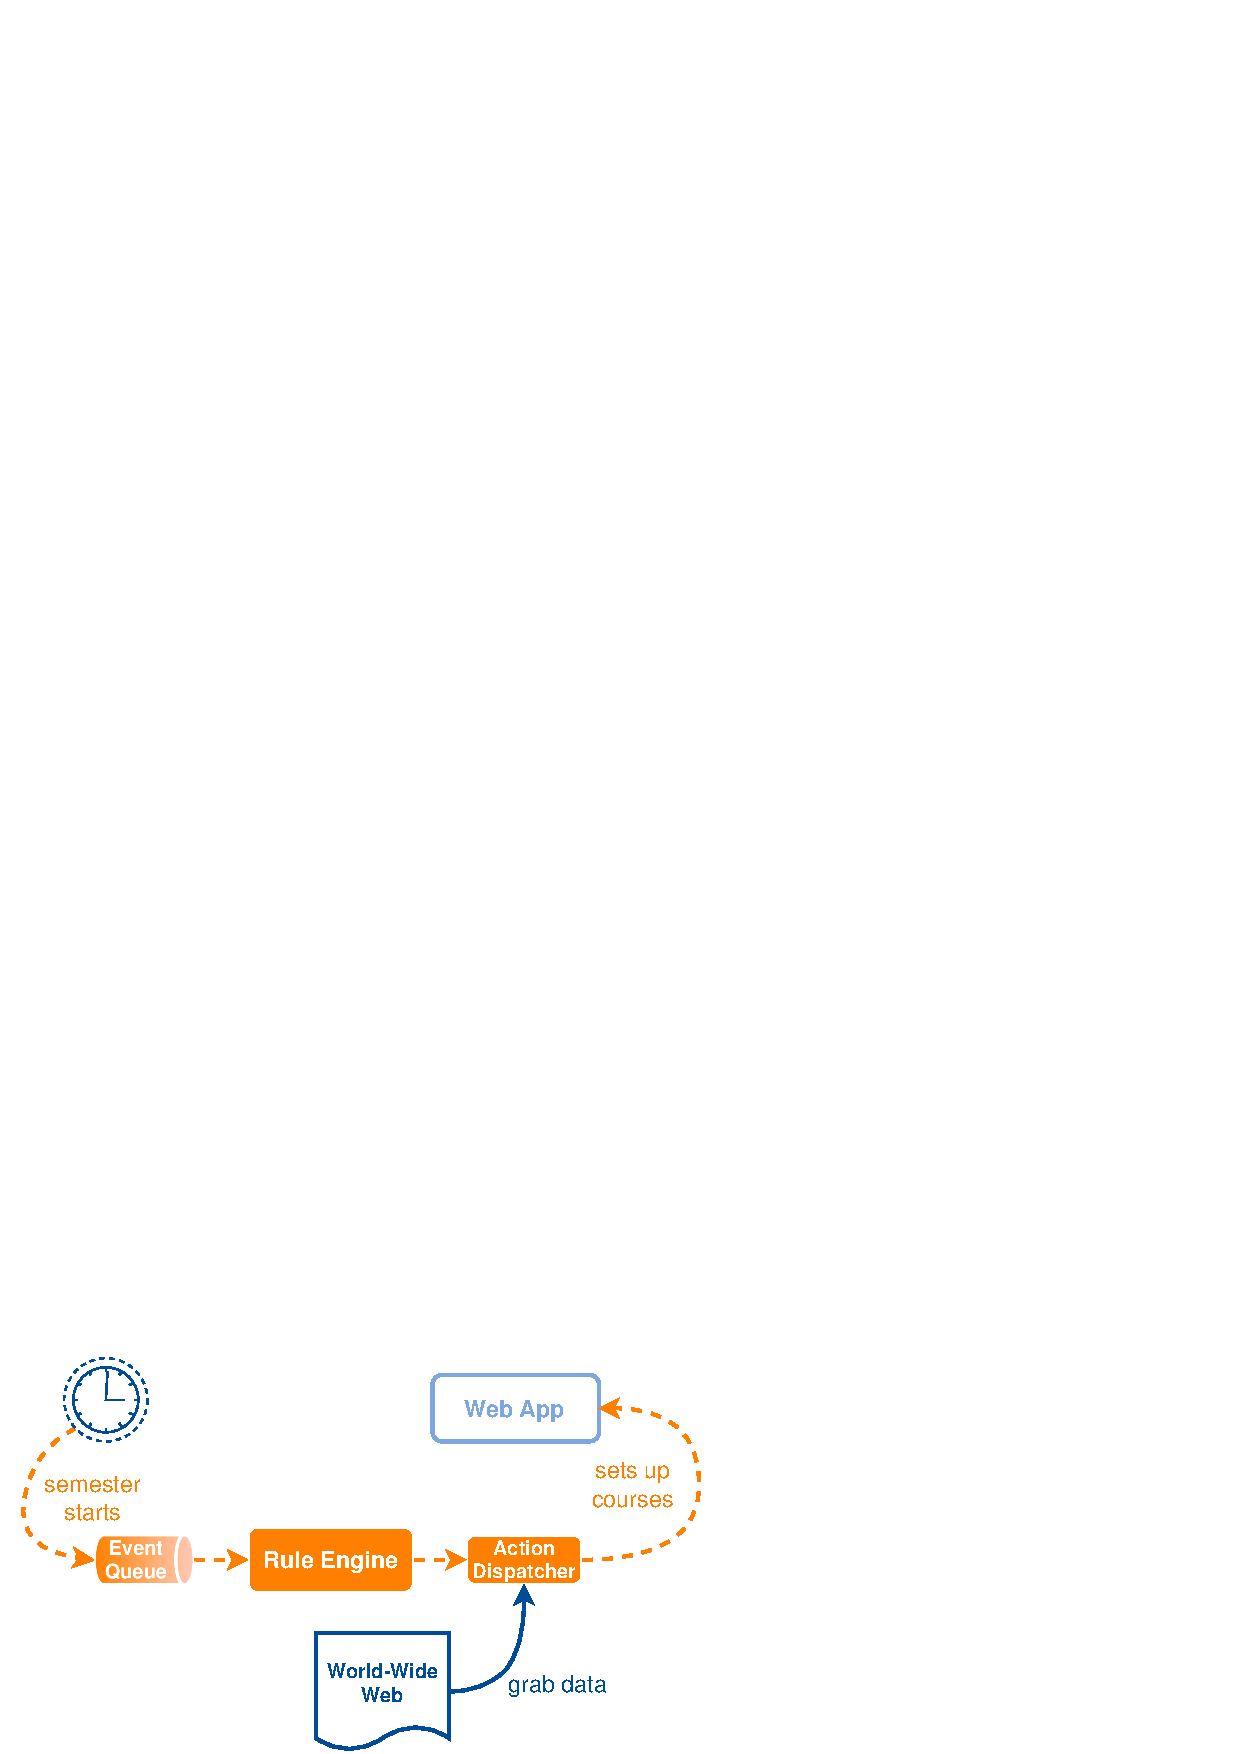
\includegraphics{figures/ProBinderCourseSetup}
  \caption{Create course resources at semester start}
  \label{fig:ProBinderCourseSetup}
\end{figure}

After setting up the semester courses, the reactive system is ready to process new student registrations for these courses.
It automatically associates students into the afore mentioned infrastructure and sets up additional infrastructure such as an exercise submission container.
Whenever a course tutor submits a new exercise to the course resource, the system will detect this and spread this information to the students, together with a deadline.
The students are expected to submit their exercise solutions before the deadline to the exercise submission container that was created reactively for them.
\begin{figure}[!ht]
  \centering
  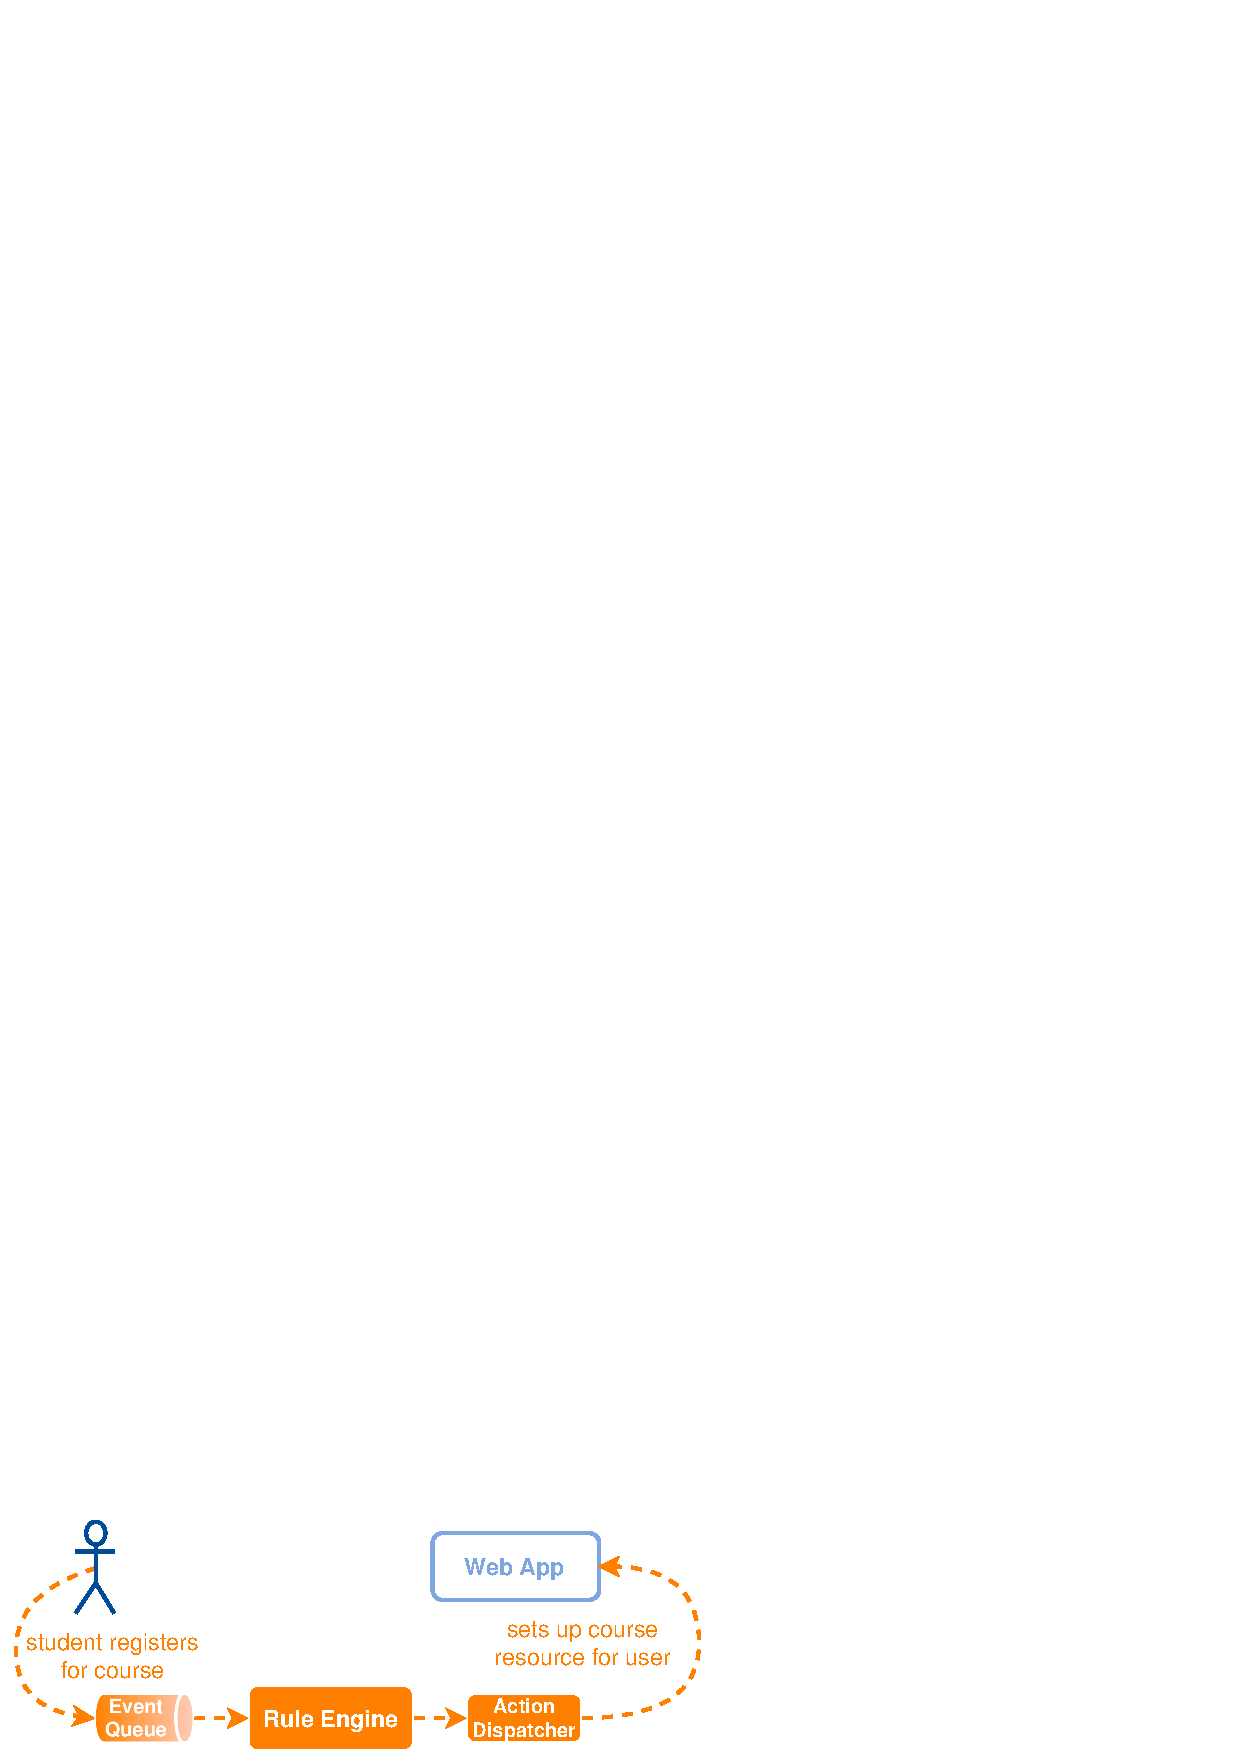
\includegraphics{figures/ProBinderStudentRegisters}
  \caption{Create course resource for registered student}
  \label{fig:ProBinderStudentRegisters}
\end{figure}

A certain amount of time before the deadline, e.g. one day, the reactive system will detect the deadline and process events that depict the current exercise submission status per student.
If the system detects a student who hasn't uploaded her exercises yet, it will notify her about the deadline.
This is an additional service that gives students the chance to react on a missed exercise submission deadline.
As soon as the deadline passed, the system will revoke write-rights to the exercise submission container and therefore disallow submissions which are too late.
\begin{figure}[!ht]
  \centering
  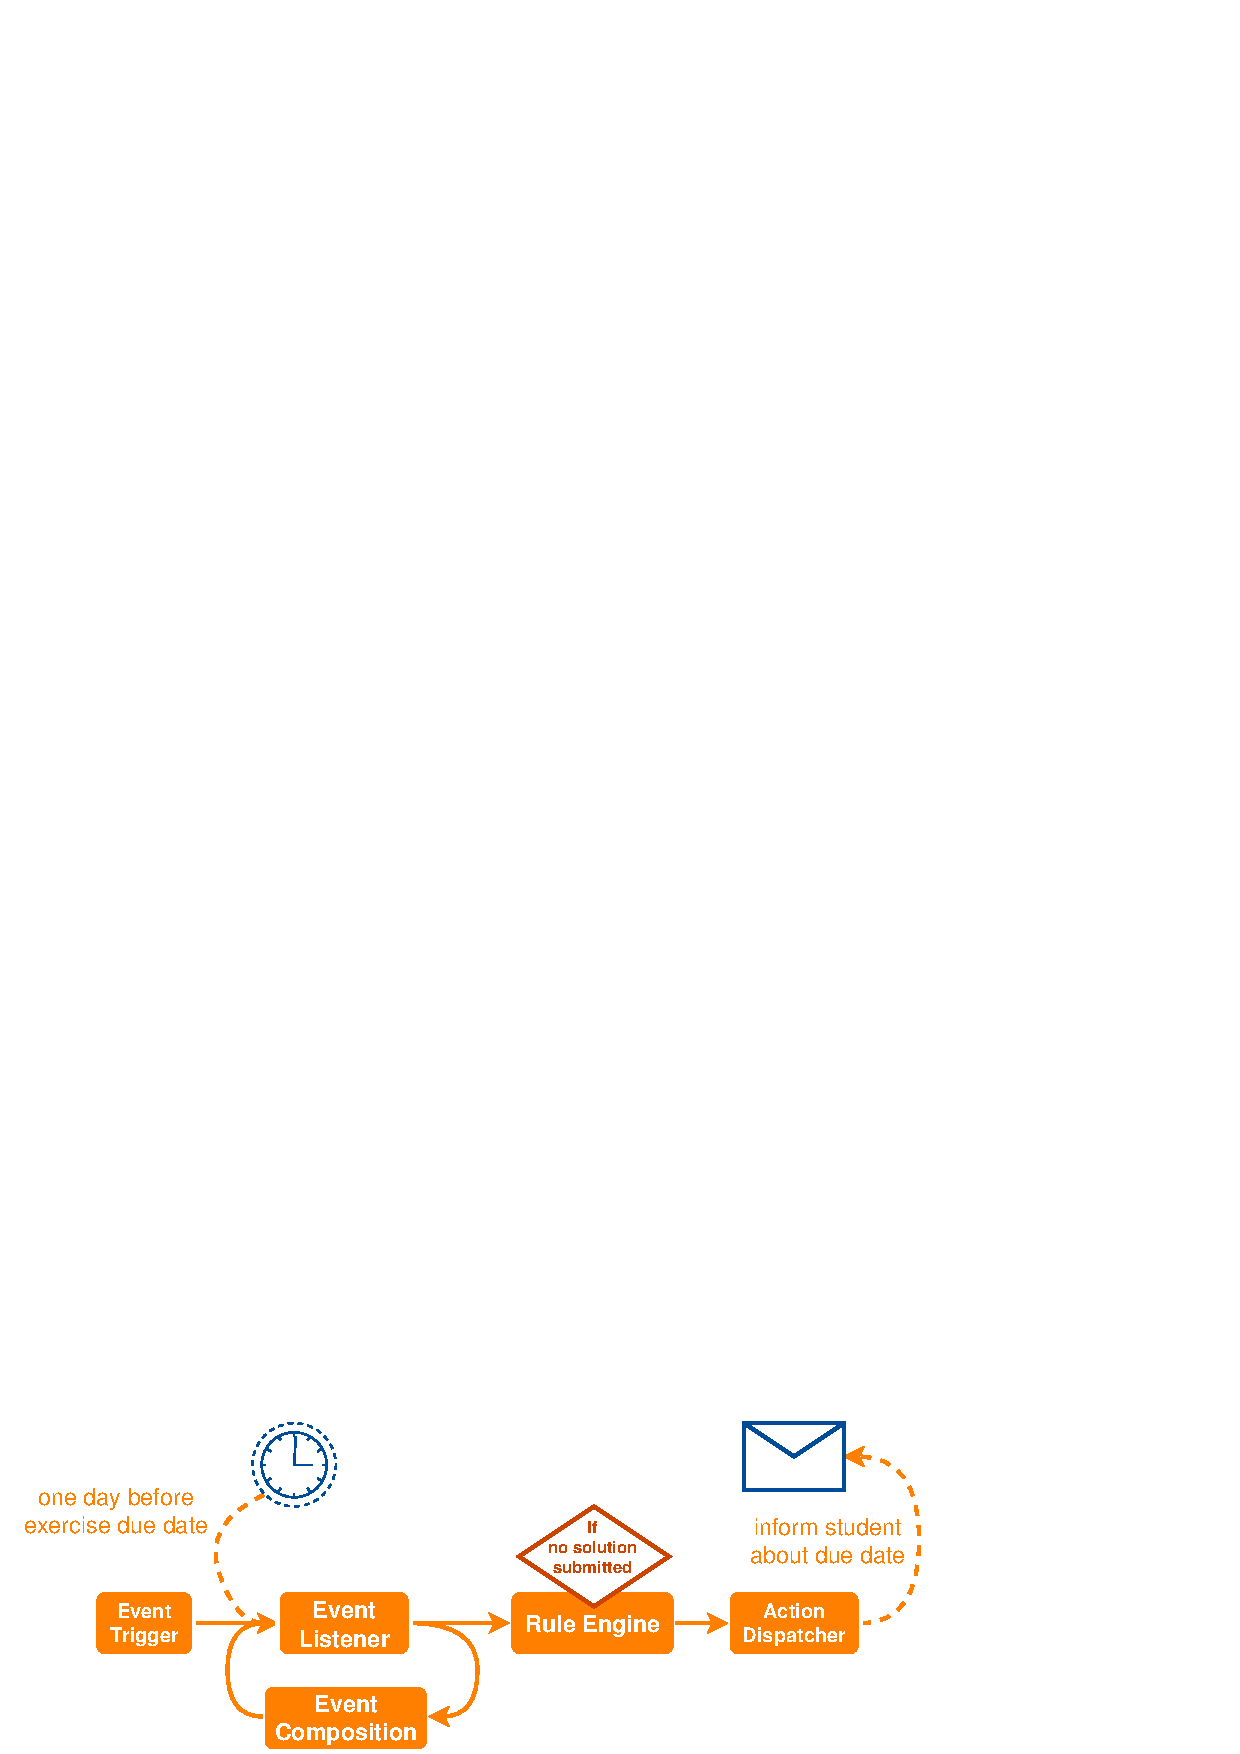
\includegraphics{figures/ProBinderExerciseNotification}
  \caption{Notify student before exercise due date}
  \label{fig:ProBinderExerciseNotification}
\end{figure}

\section{Service Functionality and Availabilty Checking}
Services offered through the Web aren't monitored or tested by users or developers from other sites.
If they rely on correct functionality or availabilty they need a way to assert this.
It is also possible that an owner of such a service doesn't have the tools to monitor his own services
Whenever such a service isn't workin correctly anymore or stops responding, these users or developers need to be able to react on this before it is too late.
With a reactive rule in place that evaluates Service Testing results, measurements can be taken early.
One action to such a failing service test could be an automatic switching of the utilized service within an action dispatcher, so that from then on it uses one which still works correctly.
\begin{figure}[!ht]
  \centering
  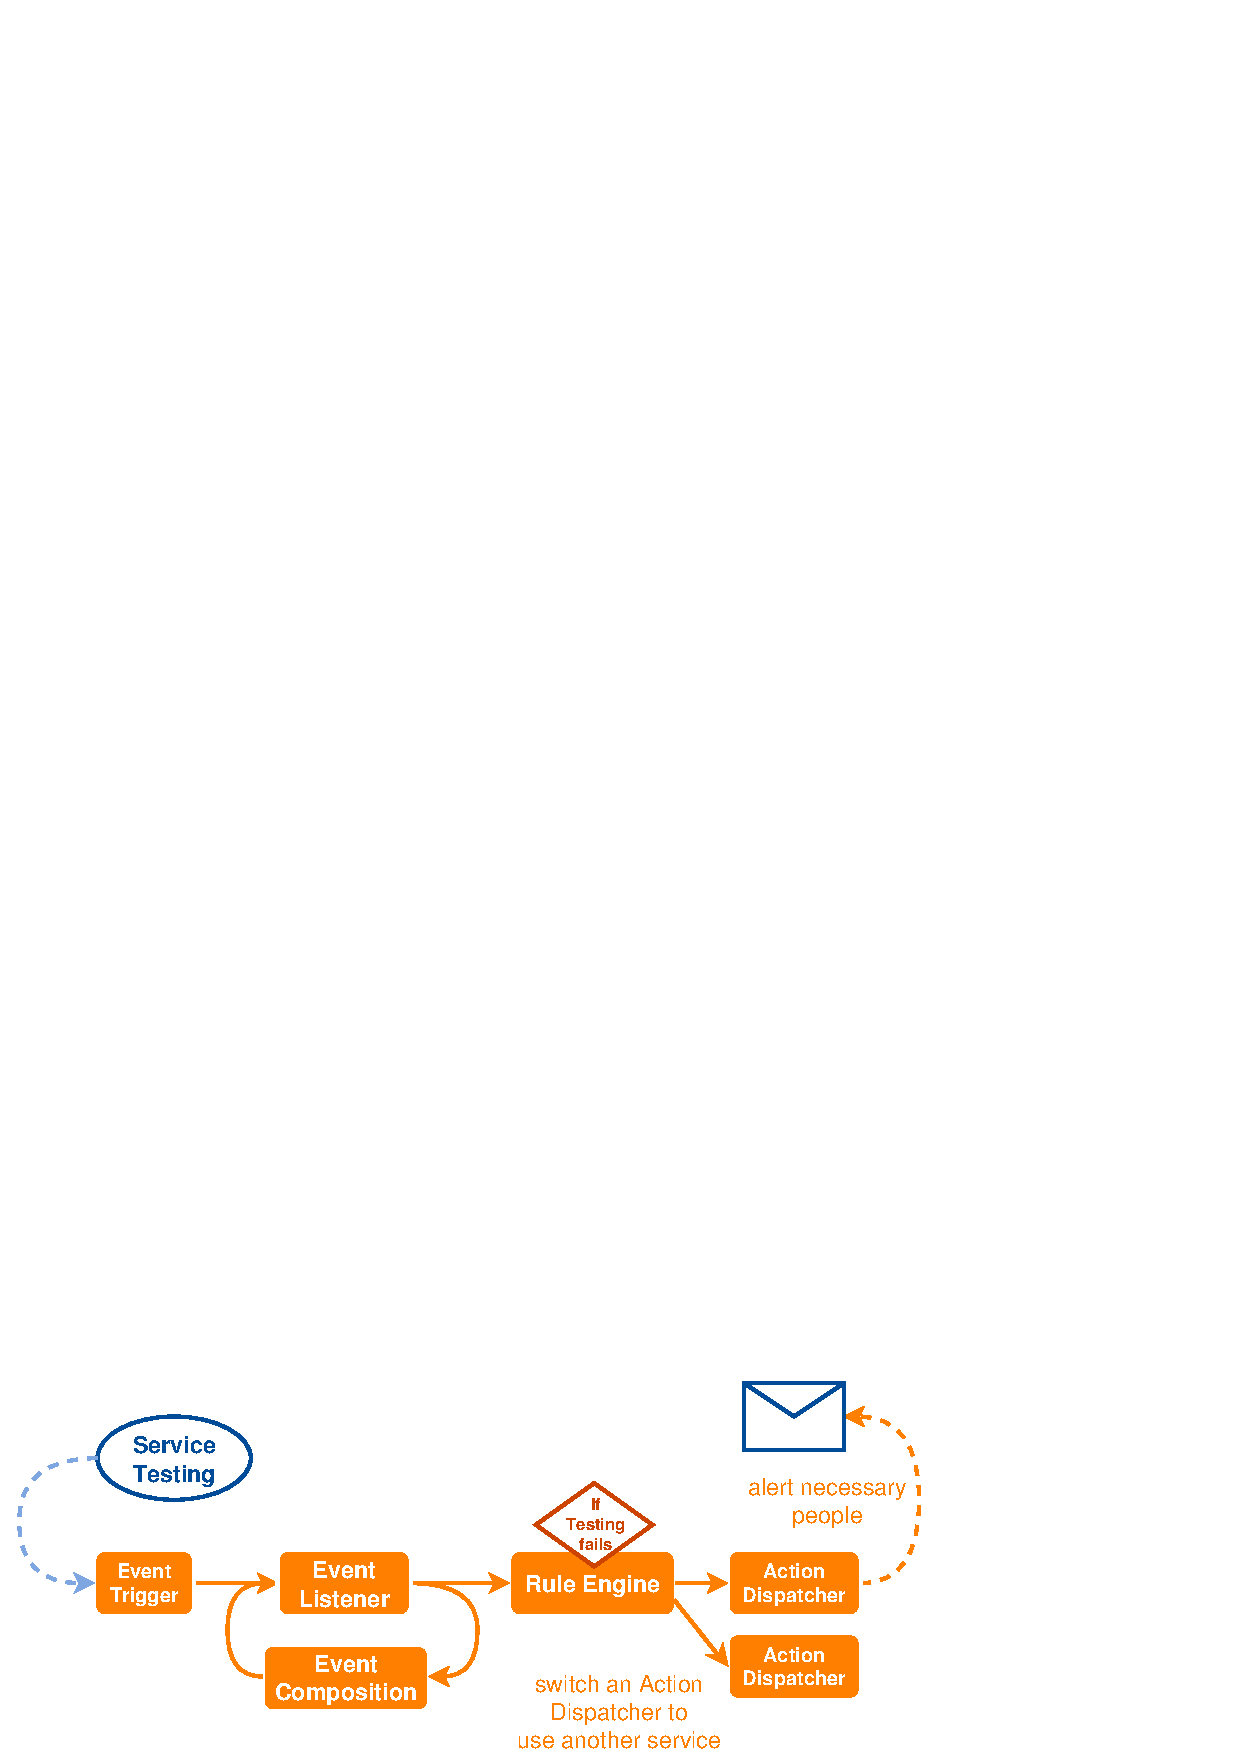
\includegraphics{figures/ProBinderServiceTesting}
  \caption{Test proper Service Functionality and Availability}
  \label{fig:ProBinderServiceTesting}
\end{figure}

\index{Web of Things}
\section{Exploiting the Web of Things}
A model for reactive information systems becomes also very interesting in the context of the \textrm{Web of Things}. 
Through the small connected devices, a lot of sensor data become accessible via the Web and can be used as events to trigger actions.
These actions could also be part of the Web of things, if there are \textrm{Things} that offer services.
One example of a reactive rule, that has parts in the \textrm{Web of Things}, is that of a server room which has a defective cooling.
The increasing temperature eventually causes the servers to shutdown or even fail.
Servers in this room could push current state information into a reactive system.
The reactive system could take measurements if it detects a certain pattern that will lead to an overheating of all systems.
It could inform certain (not so important) servers to gracefully shutdown and additionally inform administrators, who otherwise might miss the shutdown.
Even better would be if it would have the power to kick in an additional emergency cooling system to prevent the shutdown of any of the servers.
\begin{figure}[!ht]
  \centering
  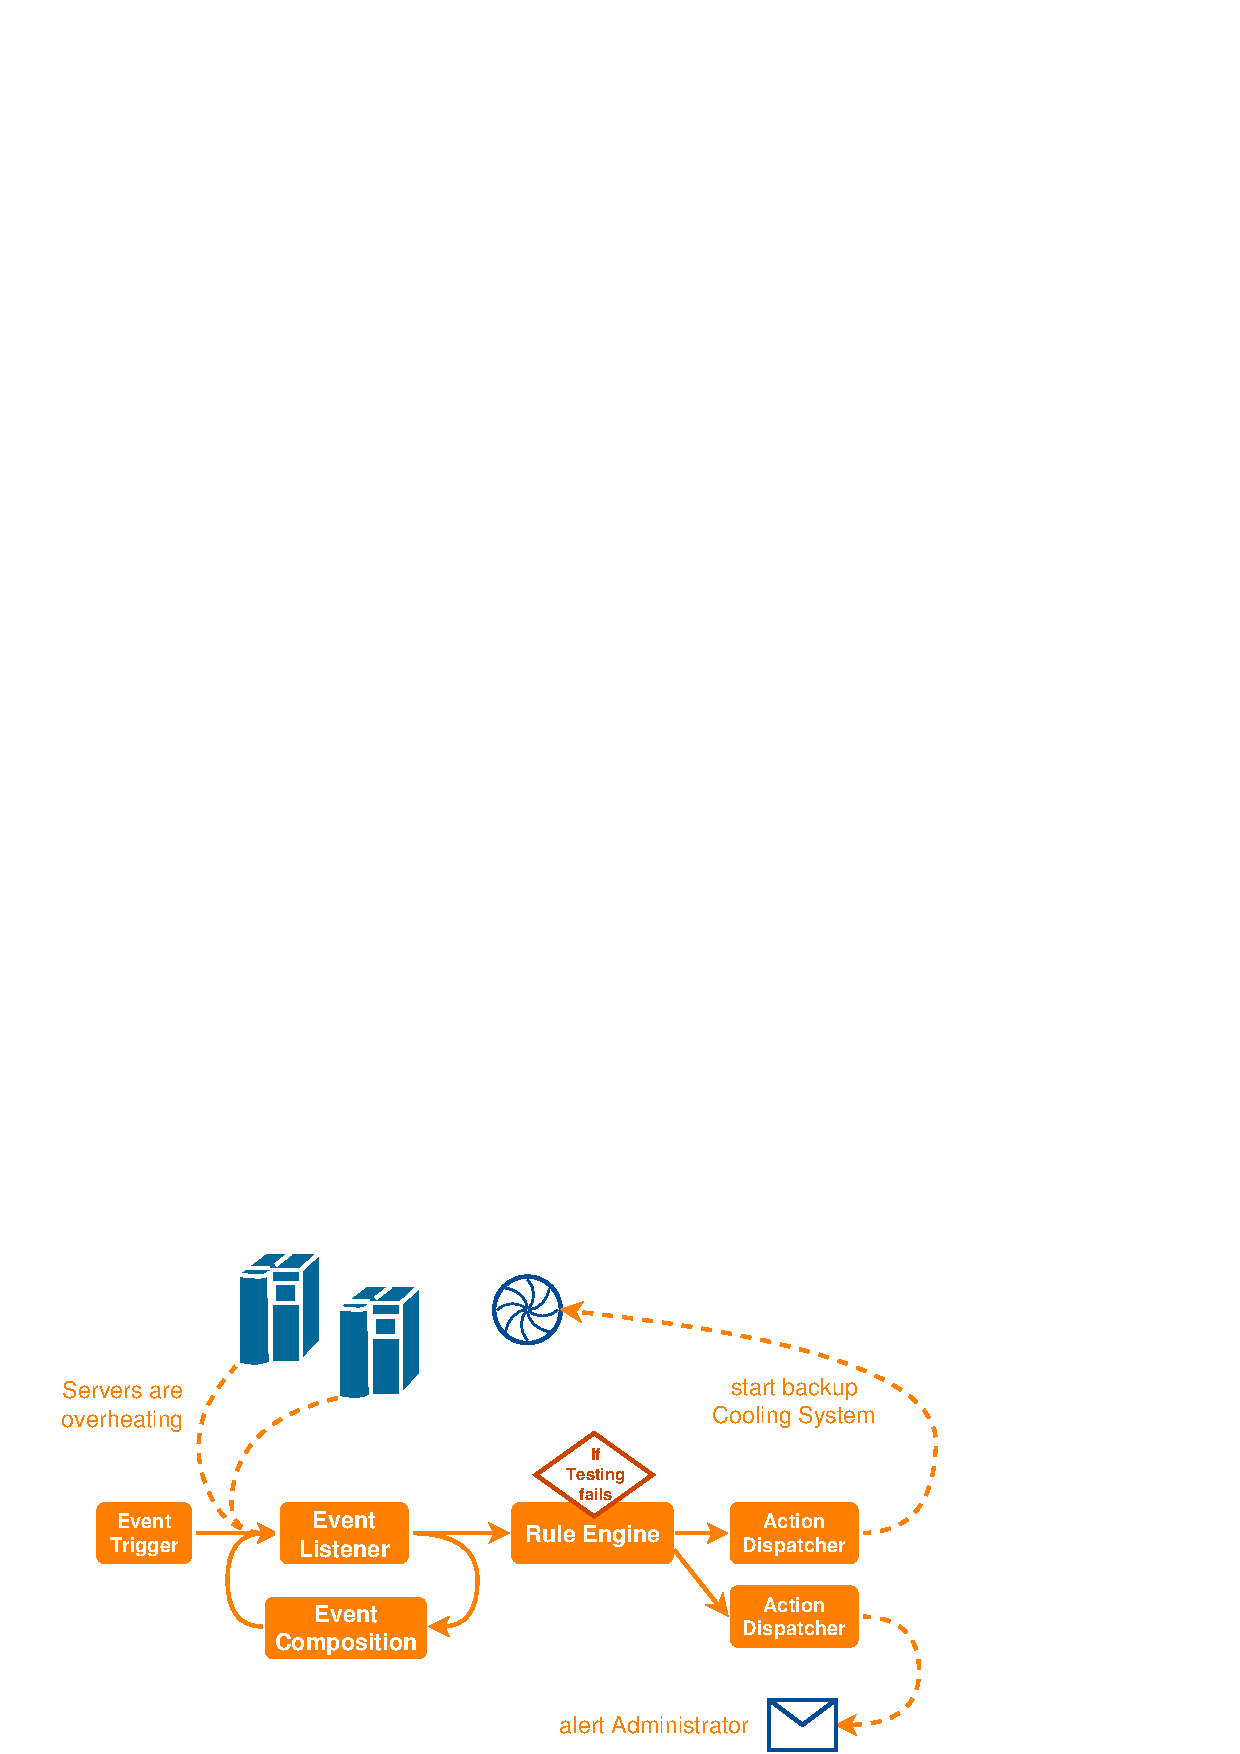
\includegraphics{figures/WoT_Server}
  \caption{Measurements on Server Failure}
  \label{fig:WoT_Server}
\end{figure}

Another scenario gets more realistic with the increasing number of homes that are connected to the Web.
A home or appartment owner has his light controls attached to the Web.
The first thing a reactive system could do, is that it detects holidays in the owner's agenda and automatically sets the light control to somewhat reasonable random during his absence.
This would make suspicious characters, which are eventually interested in his wealth, think that he's still at home.
In combination with another \textrm{Thing} that is connected to the Web and always accompanies people, the cell phone, an even more interesting application scenario can be thought of.
The phone would push location information about the owner into the system.
Whenever the owner gets close to his house, the reactive system could turn on the light in the entry area, pull up some nice music.
On a wednesday evening it could also inform the delivery service that they can deliver the owner's preferred dish now, because the owner is doing this always on a wednesday evening.
% holiday tips (Weather better somewhere else) if calendar empty

% Kalender eintrag fahrt in den süden, informaieren über offene pässe

% Regionalisierte news (news ratings)
